\chapter{Analýza}\label{ch:analýza}

\section{Bezpečnostné hrozby}\label{sec:bezpecnostne-hrozby}
\par Z hľadiska bezpečnosti väčšina firiem čelí viacerým hrozbám.
V ideálnom prostredí a vo veľkých softvérových firmách slúži na analýzu bezpečnostných hrozieb takzvaný Systém riadenia
informačnej bezpečnosti (Information Security Management System - ISMS) podľa normy ISO 27000~\cite{ISO27001:2013}.
Úlohou takéhoto systému je definovanie a spravovanie rizík, ktoré môžu vyplývať z hrozieb a zraniteľností.
Dôležitou časťou je ochrana aktív s vysokou hodnotou.
Na obrázku~\ref{fig:obr_1} je možné vidieť schému riadenia takýchto rizík.

Medzi najzákladnejšie bezpečnostné problémy napríklad patrí nezabezpečený prístup k jednotlivým projektom medzi zamestnancami.
K jednotlivým projektom v softvérovej firme by mali mať prístup iba tí zamestnanci, ktorí sa podieľajú na jeho správe a implementácii.
Vystavenie prístupových údajov, rôznych informácií o zákazníkovi a jeho používateľoch neprislúchajúcemu zamestnancovi,
môže spôsobiť veľa bezpečnostných rizík.
Napríklad zamestnanec môže zneužiť dátové úložisko nachádzajúce sa v produkcii.
Zamestnanec môže týmto spôsobom napríklad získať citlivé informácie o tržbách zákazníka alebo adrese.
Taktiež vie získať prístupové dáta k jeho koncovým zariadeniam a kompromitovať ich.
Týmto bezpečnostným rizikám prislúchajú aj možné následky nie len na strane softvérovej firmy.

\begin{figure}[H]
\begin{center}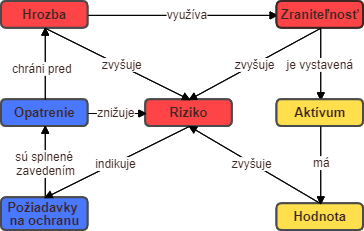
\includegraphics[width=\textwidth,height=6cm,keepaspectratio=true]{assets/risks.png}\end{center}
\caption[Prehľadová schéma riadenia rizík]{Prehľadová schéma riadenia rizík~\cite{RiskManagement}.}\label{fig:obr_1}
\end{figure}

Daný problém sa môže vyskytovať aj vo forme zlých právomocí k jednotlivým aktívam.
Softvérová firma teda môže mať navrhnutú výbornú izoláciu medzi jednotlivými projektami a zamestnancami.
Chybou môže byť aj neprimerané privilégium vo forme nadmerného prístupu k prostriedku.
Príkladom môže byť zamestnanec, ktorý nemá vo firme prístup k dátovému úložisku a jeho následnému upraveniu.
Ak nebol braný do úvahy aj prístup na prehliadanie jednotlivých údajov, takýto zamestnanec síce nevie dáta zmeniť alebo
vymazať, no je schopný prehliadať citlivé údaje a ich obsah zneužiť.

Medzi ďalšie problémy patrí takzvaná likvidácia dát.
Príkladom môže byť odchod zamestnanca z firmy.
Buďe mať stále po roku prístupy na jeho minulé projekty?
Bude mu prístup odobraný po ukončení pracovného pomeru?
Prípadne, čo ak na osobnom stretnutí prezradí prístupové údaje od bývalých projektov?
Je možné si tieto údaje útočníkom zapísať a následne sa dostať k prostriedkom?
Čo ak sa samotný zamestnanec bude chcieť po nečakanej výpovedi pomstiť napáchaním škôd?
V situácii, kedy zamestnanec nemá zrušené prístupové údaje, pričom bývalý projekt je nasadený a v praxi využívaný sa
jedná o veľmi veľké bezpečnostné riziko.

Ak sa jedná o manipuláciu so samotnými citlivými a prístupovými údajmi, tie môžu podliehať, ako bolo už spomínané neautorizovaným osobám.
Medzi najzákladnejšie riziká sú nekryptované, alebo nehašované citlivé dáta uložené v surovej forme na dátovom úložisku.
Príkladom využitia danej zraniteľnosti môže byť heslo používateľa.
Správca ani vlastník systému by nemal vedieť prístupové údaje používateľov v systéme.
Tu je možná forma zneužitia takýchto informácií k prístupu do používateľovho konta.
U systémov pracujúcich s finančnými prostriedkami, by mohlo ísť o krádež finančných prostriedkov používateľov vo vlastný prospech.

Prístup k vzdialeným zariadeniam zákazníka firmy by mala mať iba osoba, ktorá má na starosti nasadenie softvérového riešenia.
Keďže sa jedná o veľmi zodpovednú rolu vo firme, možnou hrozbou je zneužitie prístupových údajov odchytením pomocou útoku
MITM~\cite{MITM}, prípadne vyzradením údajov tretej strane podľahnutím phishing útoku~\cite{Phishing}.
Je možné sa chrániť aj proti takýmto hrozbám?

\begin{figure}[H]
\begin{center}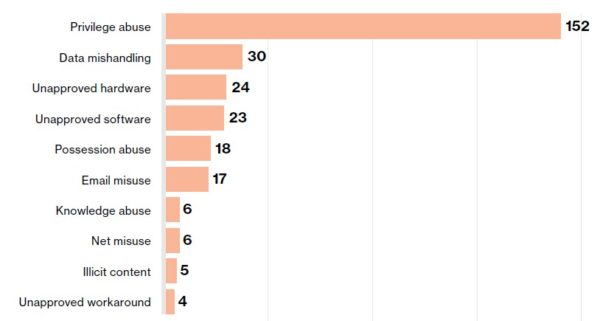
\includegraphics[width=\textwidth,height=6cm,keepaspectratio=true]{assets/priviledge_abuse.jpg}\end{center}
\caption[Najslabšie bezpečnostné miesta v softvérových firmách]{Najslabšie bezpečnostné miesta v softvérových firmách~\cite{WeaknestLink}.}\label{fig:obr_2}
\end{figure}

Ako môžme vidieť na obrázku~\ref{fig:obr_2}, najzraniteľnejším miestom v softvérových firmách je zneužitie práv zamestnancov.

\section{Súčasné opatrenia chrániace pred hrozbami}\label{sec:sucasne-opatrenia-chraniace-pred-hrozbami}

Po vymenovaní konkrétnych hrozieb a možných rizík, ktoré z nich vyplývajú je dôležité zistiť formu súčasných riešení
protiopatrení, ktoré sú schopné možné riziká odstrániť, prípadne znížiť ich naplnenie.
V praxi je nutné finančne predpovedať náklady firmy vynaložené na opatrenie a finančne predpovedať náklady možného
následku po zneužití rizika.
Ak je napáchaná škoda zo zneužitia nižšia, ako dané protiopatrenie na zamedzenie takejto formy útoku, pre softvérovú
firmu a jej zákazníkov je zamedzenie takéhoto typu hrozby z pohľadu manažmentu neoptimálne.
Z takýchto, pre firmu nepodstatných rizík je vytvorený zoznam takzvaných zvyškových rizík, pričom ich znázornenie môžme
vidieť na obrázku~\ref{fig:obr_3}.

\begin{figure}[H]
\begin{center}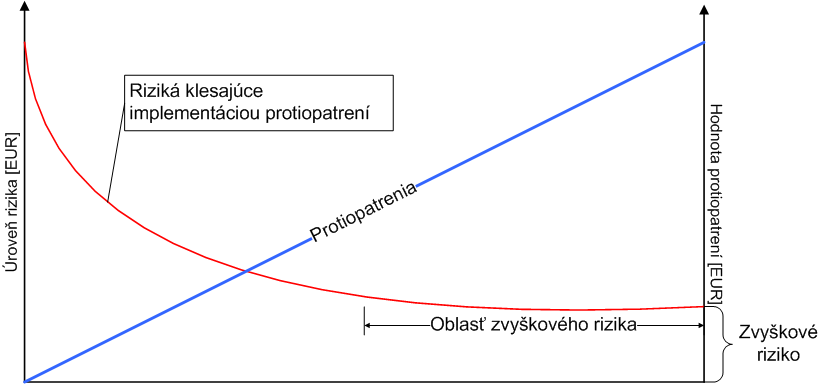
\includegraphics[width=\textwidth,height=6cm,keepaspectratio=true]{assets/zvyskove_riziko.png}\end{center}
\caption[Vizualizácia zvyškových rizík na základe hodnoty protiopatrení]{Vizualizácia zvyškových rizík na základe hodnoty protiopatrení~\cite{RiadenieRizik}.}\label{fig:obr_3}
\end{figure}

Priebeh celého procesu riadenia rizík sa vykonáva v nasledovných krokoch.
V prvom rade je nutné identifikovať riziko.
Druhým krokom je na základe druhu rizika vhodne stanoviť druh protiopatrenia.
Medzi možné spôsoby patria: Zníženie rizika, Presun rizika, Vyhnutie sa riziku, alebo zachovanie rizika.
Po validácii ošetreného rizika vznikajú podproblémy vo forme zvyškových rizík.
Tieto zvyškové riziká sú akceptované vtedy, ak nákladovosť na ich protiopatrenia sú vyššie, ako ich výška možných škôd.
Kontinuálne vykonávanie procesu riadenia rizík je možné znázorniť aj na upravenom Demingovom cykle (takzvaný model PDCA) z
bezpečnostnej normy ISO 27001~\cite{ISO27001:2013}.
Vykonávanie podľa daného modelu sa realizuje v štyroch fázach a to: Plánovať – Vykonávať – Kontrolovať – Pôsobiť.
Takýto model je možné prispôsobiť a upraviť pre potreby procesu riadenia rizík podľa obrázka~\ref{fig:obr_4} nasledovne.

\begin{figure}[H]
\begin{center}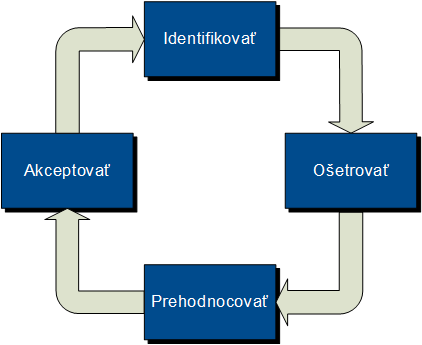
\includegraphics[width=\textwidth,height=6cm,keepaspectratio=true]{assets/pdca.png}\end{center}
\caption[Upravený PDCA model z normy ISO 27001]{Upravený PDCA model z normy ISO 27001~\cite{RiadenieRizik}.}\label{fig:obr_4}
\end{figure}

Po stručnom vysvetlení procesu riadenia rizík z pohľadu manažmentu informačnej bezpečnosti je na rade vysvetlenie
jednotlivých hrozieb spomenutých v predchádzajúcej časti práce.

Prvou hrozbou bol neautorizovaný prístup k aktívam neoprávnenými osobami.
Daný problém je z veľkej miery ovplyvnený vnútornou hierarchiou firmy.
Ak firma má v súčasnosti vytvorenú hierarchiu a každý zamestnanec má svoju špecifickú rolu na danom projekte, nutnosťou
pre zamedzenie výskytu rizík vyplývajúcich z danej hrozby je nasadenie systému autorizácie, ktorý bude jednotlivé roly
vo firme validovať, pričom prístup zamietne tým zamestnancom, ktorých rola nedovoľuje prístup k danému aktívu.

Jedným z najrelevantnejších (presne mapujúci danú hierarchiu firmy do systému) autorizačných modelov v súčasnej dobe, je riadenie prístupu na základe rolí (Role-based
access control - RBAC) podľa štandardu definovanom v ANSI/INCITS 359–2004~\cite{RBAC}.
Daný model je najčastejšie implementovaný ideológiou opatrnej bezpečnostnej politiky~\cite{OpatrnaBezpecnostnaPolitika},
ktorá spočíva v tom, že v systéme je zakázané všetko, čo nie je explicitne povolené.
Tým pádom si vieme model RBAC rozdeliť na dve časti.
Prvou je zoznam všetkých oprávnení, ktoré sú v systéme umožnené.
Druhou skupinou sú jednotlivé role, ktoré majú podľa ich významu zodpovedajúce oprávnenia.
RBAC implementácia spočíva v štyroch procesoch: Vytvorenie používateľa, vytvorenie role, priradenie role používateľovi,
a priradenie oprávnenia roli.
Jedným z problémov nastávajúcich v dynamických softvérových firmách sú výnimky vzhľadom na určité meniace sa podmienky.
Následkom výnimky vznikajú ďalšie role, ktorých počet môže byť časom neudržateľný,
pričom takto zneužité riešenie autorizovaného prístupu má za následok opätovné zvýšenie rizika zneužitia právomocí.
Jedným z možných riešení je vytvorenie dodatočnej tretej časti spočívajúcej vo vzťahu medzi samotným používateľom a oprávneniami.
Takýto vzťah by pre každého používateľa v systéme bol unikátny a nezávislý od jeho role, na rozdiel od mätúceho
vytvárania rozličných rolí s výnimkami.
Ďalšou výhodou takéhoto vzťahu je oddelenie medzi oprávneniami rolí a výnimkovými oprávneniami pre konkrétnych používateľov.

Medzi veľmi diskutované autorizačné metódy patrí riadenie prístupov na základe atribútov (Attribute-based access
control - ABAC), pričom kľúčový štandard, z ktorého ABAC vzišiel je XACML~\cite{XACML}.
Samotný koncept sa považuje za autorizačný model „novej generácie“.
Dôvodom je iný spôsob prístupu k autorizačnej problematike.
Narozdieľ od RBAC udeľovanie prístupu používateľom sa riadi na základe jednotlivých aktív, inak povedané, každej súčasti
systému~\cite{ABAC_RBAC_Attributes}.
Tento spôsob je veľmi užitočný, práve v spomínaných veľkých korporátnych softvérových firmách s veľmi výraznou dynamikou riadenia.
Pridelenie rolí používateľom teda naďalej nezávisí od ich role, ale od jednotlivých autorizačných pravidiel vyplývajúcich z namapovaných firemných aktív.
Týmto spôsobom je dokonca možné hodnotiť atribúty subjektov a zdrojov ešte pred ich zavedením do autorizačného systému.
Na druhej strane má daný koncept obmedzenie v konfigurácii, pričom určenie povolení daného používateľa je vzhľadom na návrh metódy veľmi obtiažne.
Pre danú bezpečnostnú problematiku, ktorou sa v práci zaoberáme vznikajú ďalšie nevýhody tohto riešenia a to náročnosť
implementácie a bezvýznamnosť danej metódy pre softvérové firmy menších rozmerov.
Na implementáciu daného konceptu je taktiež nutný podrobný návrh firemnej politiky~\cite{RBAC_ABAC_Encryption}.

Druhou hrozbou, ktorá so sebou prinášala veľký počet rizík bola otázka likvidácie dát.
Jednoduchým teoretickým riešením je všetky dáta a účty, ktoré už nie sú potrebné vymazať.
Realita vo firmách je žiaľ oveľa zložitejšia.
Ak zamestnanec z firmy odíde, neostane po ňom vo väčšine malých firiem iba jedno konto.
Tieto kontá a prístupové údaje bude nutné všetky vyhľadať, pričom sa vyskytujú na rôznych zariadeniach, službách technológiách a podobne.
Preto musí byť touto pracnou úlohou poverený zamestnanec z firmy, ktorému môže celý proces trvať niekoľko minút až hodín.
Takýto spôsob likvidácie dát je veľmi časovo náročný a hlavne obsahuje veľké riziko omylu a prehliadnutia niektorých z účtov.
Dané riziko nemusí explicitne vzísť iba z odchodu zamestnanca z firmy.
Zamestnancom sa počas pôsobenia v praxi môže meniť ich rola, projekty na ktorých pracujú, môže sa odstrániť služba,
ku ktorej musí mať prihlasovacie údaje a podobne.
Všetky tieto scenáre by mali byť riešené bezpečným, jednoduchým a centralizovaným spôsobom.

Jedným z riešení, ako sa vyhnúť daným rizikám je vytvorenie centrálnej autentifikácie zamestnancov.
Tým by sa zamedzilo udržiavaniu ich prihlasovacích údajov na viacerých miestach.
Jednou z možností je autentifikácia pomocou ľahkého protokolu prístupu k adresáru (Lightweight Directory Access Protocol - LDAP)~\cite{LDAP}.
Cieľom je vytvorenie servera, ktorý bude spravovať firemné prihlasovacie údaje jednotlivých zamestnancov, pričom
jednotlivé služby softvérovej firmy, ku ktorým je nutná autentifikácia budú podporovať autentifikáciu pomocou LDAP protokolu~\cite{LDAP_AUTH}.
Takéto riešenie by malo za následok správu všetkých účtov zamestnancov na jednom mieste.
Ak by nastali popísané rizikové situácie, likvidácia dát je umožnená z jednoho centralizovaného bodu.
Priebeh autentifikácie na firemné aplikácie a služby by prebiehal podľa schémy na obrázku~\ref{fig:obr_5}.

\begin{figure}[H]
\begin{center}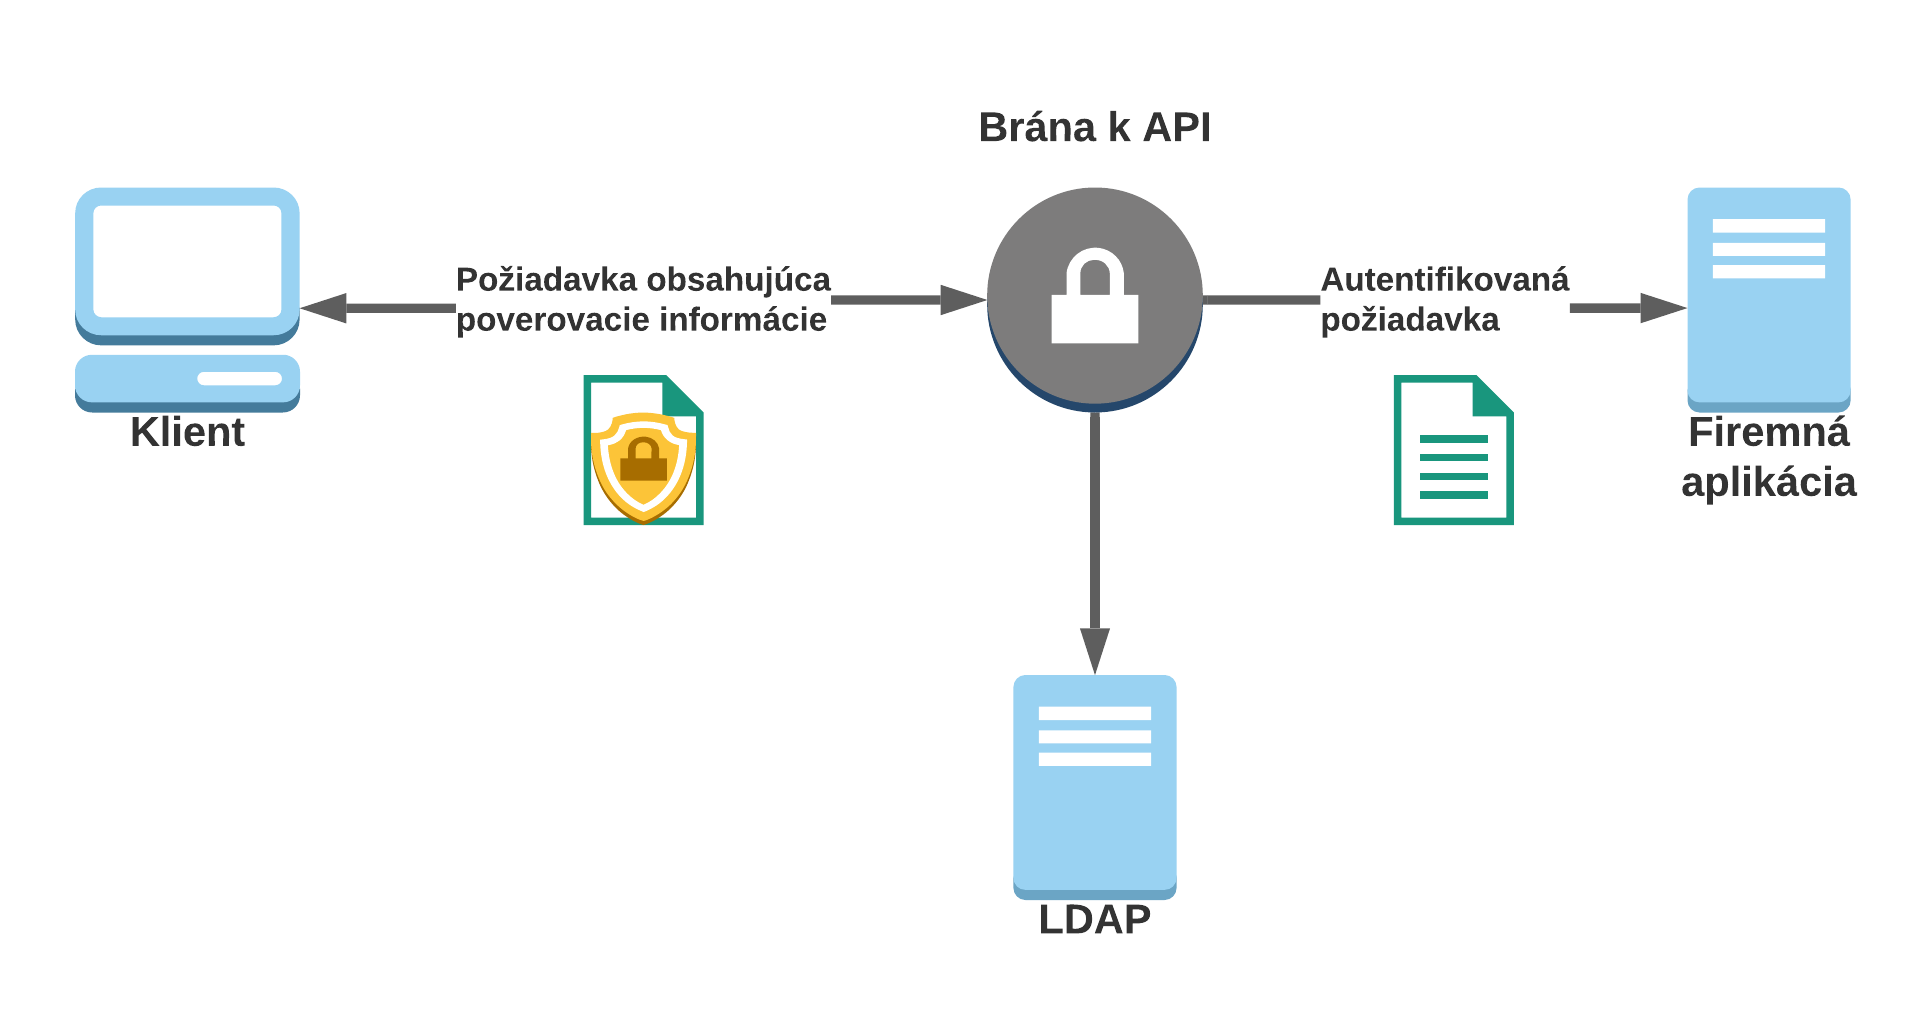
\includegraphics[width=\textwidth,height=6cm,keepaspectratio=true]{assets/ldap_schema.png}\end{center}
\caption[Schéma prihlasovania podľa protokolu LDAP]{Schéma prihlasovania podľa protokolu LDAP}\label{fig:obr_5}
\end{figure}

Treťou hrozbou bol prístup k dátam na dátovom úložisku.
Je možné dôverovať osobe s autorizáciou prehliadania dát s citlivými informáciami ako napríklad heslá, čísla kariet, prístupové adresy a podobne?
Na danú otázku existuje odpoveď vo forme modelu CIA, známeho aj ako model rozvoja bezpečnostnej politiky~\cite{CIA}.
Skratka CIA hovorí o troch dôležitých bezpečnostných pilieroch manipulácie s dátami.
Prvým z nich dôvernosť (Confidentality), ktorý hovorí o neschopnosti zistenia obsahu dôverných informácií ktorýmkoľvek používateľom.
Ako chceme dôverné informácie ochrániť pred všetkými zamestnancami, aj tými, ktorí majú k dátovému úložisku nutnú autorizáciu?
Bezpečnými spôsobmi ochrany informácií sú enkrypcia a hašovanie.
Enkrypcia je v skratke obojsmerná funkcia.
Tým pádom slúži na anonymizovanie statických dát ako napríklad informácie umožňujúce identifikáciu osôb~\cite{Encryption}.
Konkrétne sa môže jednať o dáta typu: Číslo vodičského preukazu, číslo občianskeho preukazu a podobne.
Na druhej strane hašovacia funkcia je jednosmerná.
Inak povedané, funkcia nemá možnosť spätného „odhašovania“ informácie~\cite{Hashing}.
Bezpečným prvkom, ktorý je k hašovaniu možné pridať je takzvaný „salt“, ktorý danú hašovaciu funkciu zamieša špecifickým reťazcom znakov.
Hašovacia funkcia sa používa pri druhoch informácií, ktoré sú posielané medzi dvomi sieťovými bodmi.
Napríklad môže ísť o heslo, ktorého reálnu hodnotu nikdy na strane zariadenia, ktoré ho uchováva nemusíme vedieť.
Stačí, ak sa rovnaký spôsob hašovania hesla použije na strane zariadenia vyžadujúceho autentifikáciu.
Pri procese autentifikácie sa oba haše porovnajú a ak sa rovnajú, heslá sa zhodujú.
Výsledkom hašovacej funkcie je fixne dlhý reťazec znakov.
Napríklad pri texte dlhom 250 znakov môže byť výsledný haš dlhý 32 znakov.
Preto dôležitým atribútom hašovacích funkcií je ich matematicky veľmi nízka pravdepodobnosť na vytvorenie dvoch rovnakých
výstupných reťazcov pri rozdielnych vstupoch.
Druhým pilierom modelu CIA je integrita (Integrity), ktorá hovorí o konzistencii informácií na dátovom úložisku.
Ak by došlo k ich modifikácii, vlastník daných informácií musí byť informovaný o ich zmene.
Táto skutočnosť vie ochrániť vlastníkov údajov pred ich nežiadúcou zmenou, ktorá môže byť spôsobená neautorizovaným prístupom.
Posledným pilierom modelu CIA je dostupnosť (Availability).
K skutočnej forme informácií môže mať prístup iba ich vlastník a to v čitateľnej a konečnej podobe.
To napríklad znamená, že pred zobrazením používateľovho rodného čísla musí byť táto enkryptovaná dôverná informácia
spätne dekryptovaná do originálnej podoby.

Posledný spomínaný problém nesie so sebou výskyt rizík v podobe získania prístupových údajov, či už sa jedná o autentifikáciu
do firemného systému, alebo dáta potrebné na nasadenie finálneho softvérového produktu ku koncovým zariadeniam zákazníkov.
V oboch prípadoch, ako bolo už spomenuté ide o veľmi vážne bezpečnostné riziká, keďže sa taktiež priamo týkajú zákazníkov
softvérovej firmy.
Pre šifrovaný spôsob komunikácie je potrebné implementovať komunikačné protokoly v súlade s bezpečnostnými požiadavkami.
Komunikácia medzi vzdialeným webovým firemným serverom a zamestnancom by mohla prebiehať cez zabezpečený protokol
HTTPS (Hypertext transfer protocol secure)~\cite{HTTPS}, kde by boli jednotlivé autentifikačné dáta na transportnej vrstve
šifrované bezpečnostným protokolom TLS (Transport Layer Security)~\cite{TLS}.
Samotný spôsob autentifikácie by mohol byť uskutočnený podľa formátu JWT (JSON Web Token), spolu s využitím autentifikačného
protokolu OAUTH(2.0) (Open standard for access delegation)~\cite{JWT}.
Keďže prístup k firemným zdrojom je veľmi diskrétny, z bezpečnostného hľadiska je odporúčané použitie dvojfaktorovej
autentifikácie~\cite{DvojfaktorovaAutentifikacia}, ktorej priebeh môžme vidieť na obrázku~\ref{fig:obr_6}.
Dvojfaktorová autentifikácia nepodlieha útokom hrubou silou a taktiež po získaní prístupových dát napríklad odchytením,
alebo inou formou útoku nepodlieha ich zneužitiu z dôvodu veľmi frekventovane meniaceho sa unikátneho verifikačného kódu.
Pokiaľ sa jedná o komunikáciu medzi koncovými zariadeniami zákazníkov, tú je možné zabezpečiť protokolom SFTP (SSH File
Transfer Protocol)~\cite{SFTP}, ktorý umožňuje posielanie súborov cez protokol SSH (Secure Shell)~\cite{SSH}, slúžiaci
na bezpečné vykonávanie príkazov na vzdialených zariadeniach.

\begin{figure}[H]
\begin{center}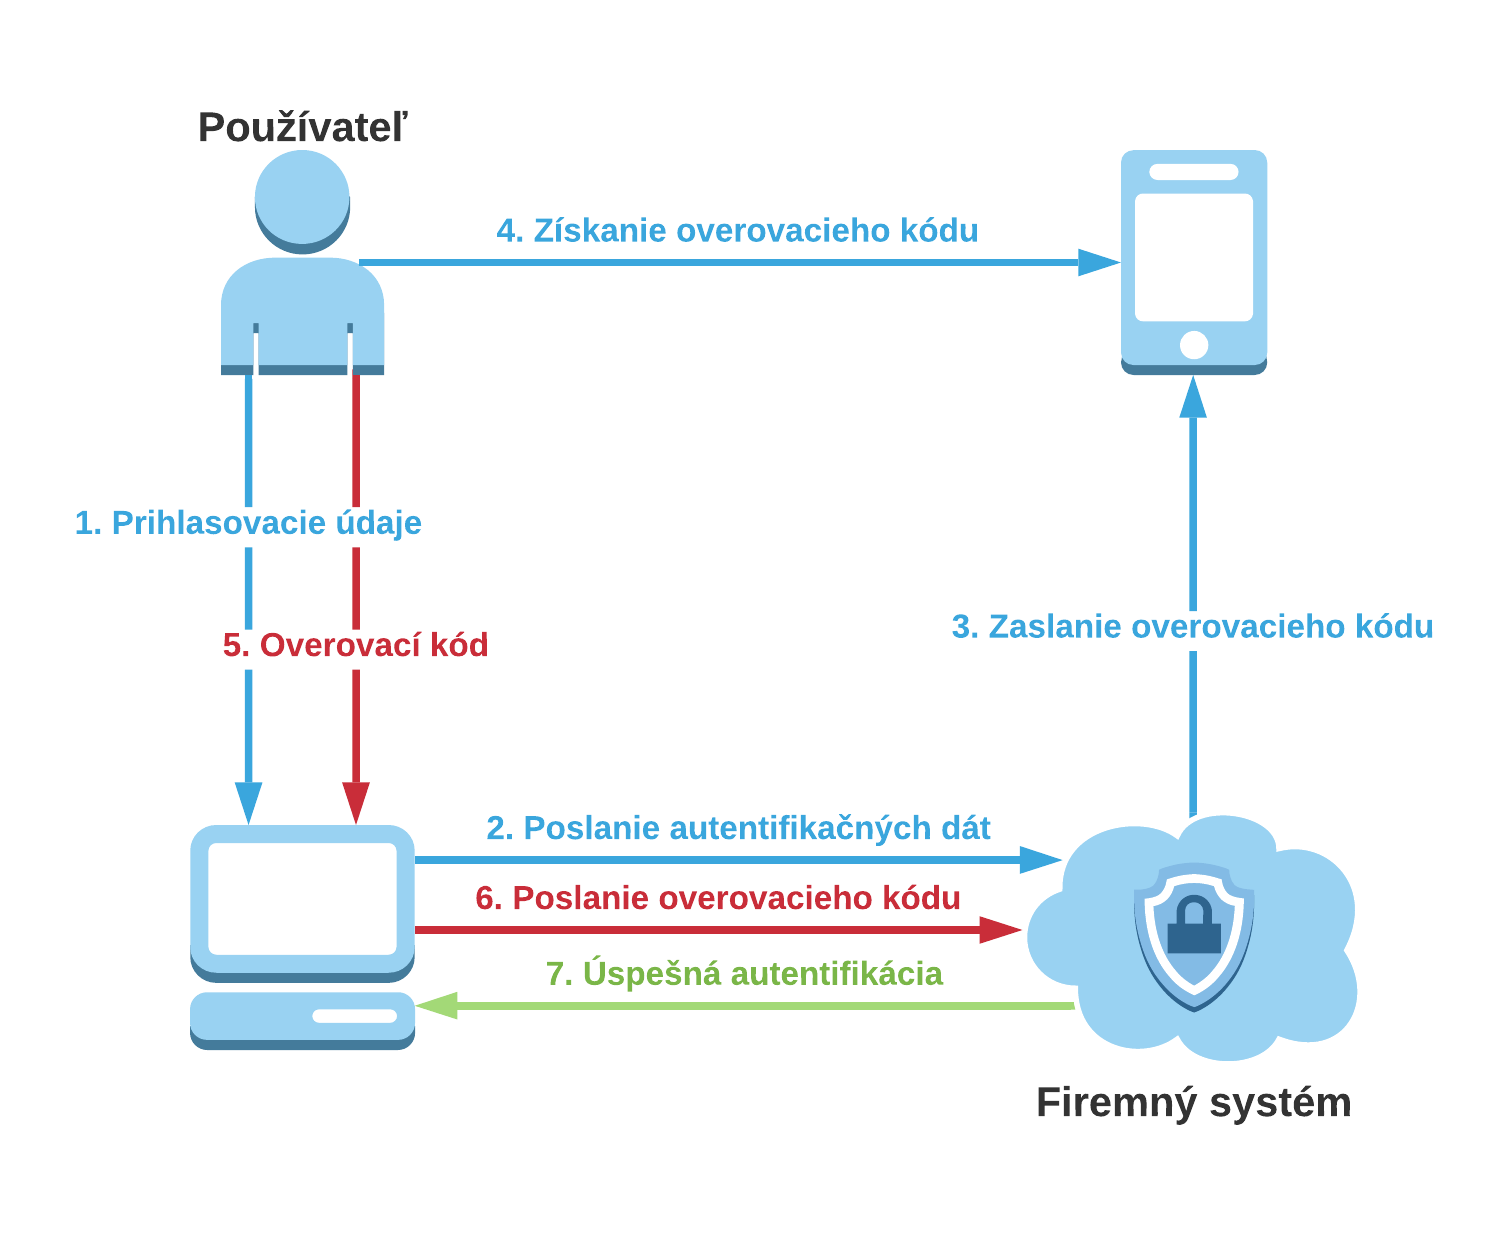
\includegraphics[width=\textwidth,height=8cm,keepaspectratio=true]{assets/2fa_auth.png}\end{center}
\caption[Schéma dvojfaktorovej autentifikácie]{Schéma dvojfaktorovej autentifikácie}\label{fig:obr_6}
\end{figure}

\section{Protokol SSH}\label{sec:protokol-ssh}

Komunikácia pri nasadzovaní softvéru, alebo vzdialený prístup na koncové zariadenie zákazníka je možné realizovať v
oboch prípadoch cez protokol SSH~\cite{SSH}.
Z toho dôvodu je potrebné dôkladne rozobrať, ako daný protokol funguje, aké má možnosti využitia, bezpečnosť a druhy
nastavenia.
SSH, tiež známy, ako „Secure Shell“ alebo „Secure Socket Shell“, je sieťový protokol patriaci podľa modelu OSI do aplikačnej
vrstvy~\cite{OsiModel}.
Pomocou širokej množiny rôznych šifrovacích technológií poskytuje možnosti na vytvorenie kryptograficky zabezpečeného
spojenia a tým pádom bezpečnej komunikácie medzi dvoma vzdialenými bodmi (klient - server)~\cite{SshWorkflow}.
Uľahčenie bezpečnej komunikácie medzi dvoma bodmi zabezpečuje transportná vrstva, ktorá zvyčajne operuje nad TCP / IP
modelom a navyše poskytuje kompresiu a urýchľuje prenos informácií~\cite{SshSecurity}.
Na zabezpečenie prenosu informácií medzi klientom a serverom sa využíva viacero metód, ako napríklad: symetrické šifrovanie,
asymetrické šifrovanie alebo hašovanie.

\subsection{Symetrické šifrovanie}\label{subsec:symetricke-sifrovanie}

Symetrické šifrovanie umožňuje použitie iba jedného kľúča na šifrovanie správ posielaných druhej strane a následné
dešifrovanie odpovedí poslaných naspäť.
Tým pádom ktokoľvek, kto je držiteľom kľúča, môže šifrovať a dešifrovať správy komukoľvek inému, kto drží ten istý kľúč.
K vytvoreniu kľúča prispievajú vždy obe strany, pričom výsledné tajomstvo nie je externým stranám nikdy známe.
Tajný kľúč sa vytvára pomocou procesu známeho, ako algoritmus výmeny kľúčov.
Táto výmena vedie k tomu, že server a klient dospejú k rovnakému kľúču nezávisle od seba.
Tento proces je možné uskutočniť zdieľaním určitých častí verejných údajov a ich následnou manipuláciou.
SSH je možné nakonfigurovať tak, aby využíval rôzne symetrické šifrovacie systémy, vrátane AES, Blowfish, 3DES, CAST128 a
Arcfour~\cite{SshEncryption}.
Server aj klient môžu rozhodnúť o zozname podporovaných šifier, zoradených podľa preferencie.
Pri nadviazaní pripojenia medzi bodmi, klient serveru pošle zoznam šifrovacích algoritmov zoradených podľa preferencie.
Prvá možnosť zo zaslaného zoznamu, ktorá je nastavená ako preferencia na serveri sa následne použije ako algoritmus
symetrického šifrovania.
Na obrázku~\ref{fig:obr_7} je graficky znázornená schéma bezpečného nadviazania pripojenia cez SSH protokol.

\begin{figure}[H]
\begin{center}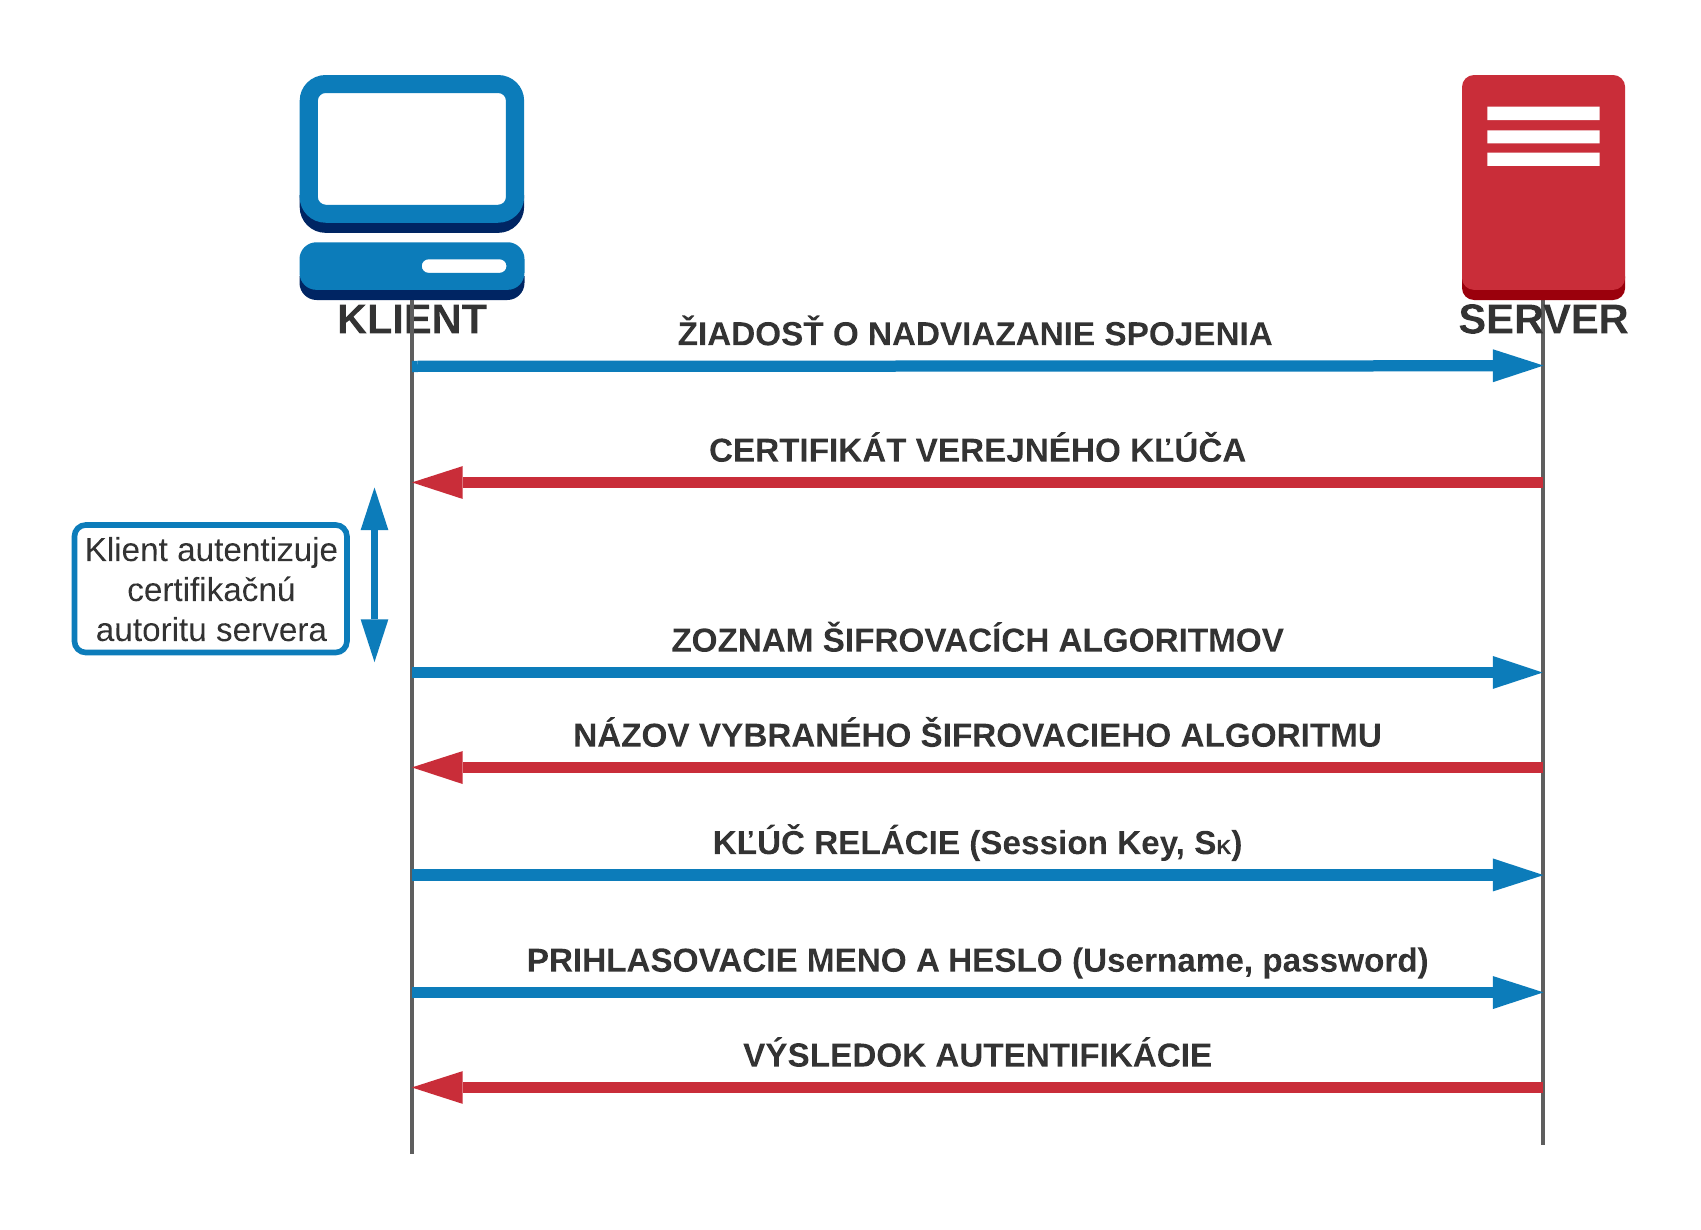
\includegraphics[width=\textwidth,height=8cm,keepaspectratio=true]{assets/symmetric_ssh.png}\end{center}
\caption[Schéma bezpečného nadviazania SSH pripojenia]{Schéma bezpečného nadviazania SSH pripojenia}\label{fig:obr_7}
\end{figure}

\subsection{Asymetrické šifrovanie}\label{subsec:asymetricke-sifrovanie}

Asymetrické šifrovanie sa líši od symetrického tým, že na odoslanie údajov sú potrebné dva súvisiace kľúče.
Jeden z týchto kľúčov je známy ako súkromný kľúč (private key), zatiaľ čo druhý sa nazýva verejný kľúč (public key)~\cite{SshEncryption}.

Verejný kľúč je možno ľubovoľne zdieľať s druhou stranou komunikácie, pričom je „spárovaný“ so súkromným kľúčom.
Matematický vzťah, ktorý oba kľúče spolu „spároval“ umožňuje verejnému kľúču šifrovať správy, ktoré je možné dešifrovať
iba pomocou súkromného kľúča, pričom je nemožné odvodiť súkromný kľúč z verejného.
Toto je jednosmerná schopnosť, čo znamená, že verejný kľúč nemá schopnosť dešifrovať správy, ktoré píše, ani dešifrovať
prijaté správy šifrované súkromným kľúčom.

Aby paradigma verejného kľúča fungovala, súkromný kľúč nesmie byť zdieľaný s inou stranou komunikácie.
Súkromný kľúč je jediný komponent schopný dešifrovať správy, ktoré boli šifrované pomocou priradeného verejného kľúča.
Na základe tejto skutočnosti každá entita schopná dešifrovať tieto správy preukázala, že má kontrolu nad súkromným kľúčom.

Asymetrické šifrovanie je využívané pri procesoch, ako napríklad počiatočná výmena kľúčov, ktorý sa používa na nastavenie
symetrického šifrovania pri šifrovaní relácie (session).
V tejto fáze obe komunikujúce strany vytvárajú dočasné páry kľúčov pri výmene verejného kľúča, aby vytvorili spoločné tajomstvo.

\subsection{Hašovanie}\label{subsec:hasovanie}

Ďalšou formou zabezpečenia komunikácie, ktorú SSH využíva, je kryptografická hašovacia funkcia.
Kryptografická hašovacia funkcia používa jednosmerné matematické funkcie, ktoré sa dajú ľahko vypočítať na vygenerovanie
hašovacej hodnoty zo vstupu, pričom je veľmi náročné reprodukovať pôvodný vstup vykonaním výpočtov na už vygenerovanom haši.
Použitie rovnakej hašovacej funkcie a správy by malo vytvoriť rovnaký výstup, pričom úprava ktorejkoľvek časti údajov by
mala vytvoriť výstup úplne iný~\cite{EDGAR201733}.
Používateľ by nemal byť schopný vyrobiť pôvodnú správu z daného zahešovaného výstupu, no mal by byť schopný zistiť, či daná správa
vyprodukovala daný haš.
Vzhľadom na tieto vlastnosti sa haše používajú hlavne na účely integrity údajov a na overenie autenticity komunikácie~\cite{SshEncryption}.

\subsection{Autentifikácia}\label{subsec:autentifikacia}

Akonáhle transportná vrstva vytvorí bezpečný komunikačný tunel na prenos informácií medzi koncovými bodmi, server klientovi
ponúkne spôsoby autentifikácie, ktoré podporuje.
Príkladom spôsobu autentifikácie je použite podpisu kódovaného súkromným kľúčom alebo zadanie hesla.
Klient sa potom pokúsi autentifikovať pomocou ktorejkoľvek z podporovaných metód.

Servery môžu byť nakonfigurované tak, aby umožňovali rôzne typy autentifikácie, čo dáva každej strane značnú mieru flexibility.
Z implementácie servera vyplývajú podporované metódy šifrovania, spomedzi ktorých si klient môže zvoliť poradie metód autentifikácie.
Keďže heslo je pri pohybe po transportnej vrstve šifrované, je možné ho bezpečne odoslať v akejkoľvek sieti~\cite{SshSecurity}.

\subsection{Pripojenie}\label{subsec:pripojenie}

Po úspešnej autentifikácii cez transportnú vrstvu je možné otvoriť medzi danými komunikačnými entitami viac kanálov multiplexovaním\footnote{Multiplexovanie
pripojenia umožňuje pracovať s viacerými reláciami (sessions) cez jedno pripojenie TCP~\cite{SshSecurity}.} spojenia.

Multiplexovanie nastáva z dôvodu, aby sa rôzne typy relácií navzájom neovplyvňovali a aby bolo možné po ukončení relácie
uzavieť jej kanál bez prerušenia primárneho spojenia SSH.

Každý komunikačný kanál má svoje unikátne číslo, pričom klient aj server si môžu vytvoriť toľko kanálov, koľko potrebujú.

\section{Dôvernosť informácií}\label{sec:dovernost-informacii}

Ako bolo spomenuté vyššie, dôvernosť informácií je jedným z hlavných aspektov informačnej bezpečnosti.
Na zabezpečenie dôvernosti informácií (taktiež ako u spomínaného protokolu SSH vyššie) slúži šifrovanie.
Jednými z najbezpečnejších a najširšie používaných šifrovacích algoritmov sa stali algoritmy pod štandardom AES (Advanced Encryption Standard).

Počiatky AES siahajú do roku 1999, kde Národný inštitút pre štandardy a technológie (National Institute of Standards and Technology -
NIST) vybral z pätnástich návrhov šifrovacích algoritmov podrobených svetovou kryptografickou komunitou vrátane Národnej
bezpečnostnej agentúry (National Security Agency - NSA) iba päť algoritmov na rozsiahlejšiu analýzu~\cite{AdvancedEncryptionStandard}:

\begin{itemize}
    \item \textbf{MARS}, predložený veľkým tímom spoločnosti IBM Research.
    \item \textbf{RC6}, predložené spoločnosťou RSA Security.
    \item \textbf{Rijndael}, predložené dvoma belgickými kryptografmi, Joan Daemen a Vincent Rijmen.
    \item \textbf{Serpent}, predložili: Ross Anderson, Eli Biham a Lars Knudsen.
    \item \textbf{Twofish}, predložený veľkým tímom výskumníkov z Counterpane Internet Security, vrátane významného kryptografa Brucea Schneiera.
\end{itemize}

Po mnohých spätných väzbách, debatách a analýzach bola šifra Rijndael vybraná ako navrhovaný algoritmus pre AES v
októbri 2000.
Následne bol AES v roku 2002 publikovaný Národným inštitútom pre štandardy a technológie a následne schválený Národnou bezpečnostnou
agentúrou (NSA) pre prácu s prísne tajnými informáciami (FIPS) PUB 197.
Vďaka otvoreným autorským právam sa stal AES priemyselným štandardom šifrovania~\cite{UnderstandingAes}.

AES je symetrická kľúčová šifra.
Z toho dôvodu sa na šifrovanie a dešifrovanie používa rovnaký kľúč.
Asymetrické kľúče sú najvhodnejšie na prenos externých súborov, zatiaľ čo symetrické kľúče sú vhodnejšie na interné
šifrovanie.
Výhodou symetrických systémov, ako AES je ich rýchlosť, pretože algoritmus symetrického kľúča vyžaduje menší výpočtový
výkon ako asymetrický, vďaka čomu je jeho spustenie rýchlejšie a efektívnejšie~\cite{UnderstandingAes}.

Šifry spadajúce pod štandard AES sú tiež charakterizované ako blokové šifry.
Pri týchto typoch šifier je vstup (informácia, ktorá sa má zašifrovať), rozdelený do sekcií nazývaných bloky.
AES používa rôznu veľkosť blokov, ako napríklad: 128, 192 alebo 256 bitov, pričom veľkosť bloku 128 bitov je optimálnym
kompromisom medzi rýchlosťou a bezpečnosťou šifrovania.
Pri šifrovaní o veľkosti bloku 128 bitov sú dáta rozdelené do dvojrozmernej matice o rozmeroch štyri stĺpce a štyri riadky,
ktorá obsahuje 4 * 4 = 16 bajtov.
Pretože na bajt je osem bitov, celkový počet v každom bloku je 128 bitov, pričom veľkosť šifrovaných údajov zostáva
rovnaká: 128 bitov holého textu poskytne 128 bitov šifrovaného textu~\cite{rfc3602}.

AES šifra má viacero prevedení, pričom jedno z možných rozdelení šifier v AES štandarde je podľa deterministických výstupov.
Pri nedeterministických prevedeniach majú dva rovnaké vstupy po zašifrovaní dva rozdielne výstupy, kde pri deterministickom
prevedení je rovnaký výstup pri rovnakých vstupoch garantovaný.

AES obsahuje viacero variant šifrovania, kde jednou z variant je režim šifrovanej spätnej väzby (The cipher feedback - CFB),
ktorý spracuje výstupy nedeterministickým spôsobom.
Tým pádom je z pohľadu bezpečnosti daný variant veľmi dobre uplatniteľný pri šifrovaní osobných údajov~\cite{CFB}.
Na druhej strane deterministické výstupy sú napríklad uskutočniteľné pomocou takzvaného Vektora syntetickej inicializácie
(Synthetic Initialization Vector - SIV)~\cite{SIV}, kde takýto typ výstupov je vhodný na kontrolu prístupových údajov, ktorých obsah je
utajený, no konzistencia výstupov sa dá skontrolovať.
Jedným z príkladov takéhoto spôsobu šifrovania je možnosť overenia totožnosti komunikujúcej entity.

\section{Existujúce riešenia}\label{sec:existujuce-riesenia}

\subsection{AWS Secrets Manager}\label{subsec:aws-secrets-manager}

AWS Secrets Manager je službou cloudovej platformy Amazon Web Services, ktorá má za úlohu bezpečné ukladanie citlivých údajov.
Služba je reprezentovaná vo forme API rozhrania.
Tým pádom sú operácie nad citlivými dátami aplikácie vo forme šifrovaných HTTPS požiadaviek na dané API rozhranie.
Hlavnou úlohou tohto riešenia je predovšetkým zamedzenie odhalenia citlivých údajov v zdrojovom kóde, ako napríklad prístupové údaje.

Dátové úložisko s citlivými údajmi prislúchajúce pod správu služby AWS Secrets Manager sa nachádza na cloudovom serveri, ktorý
je prístupný iba oprávneným používateľom.
Secrets Manager taktiež zabezpečuje správu rolí a oprávnení v systéme, alebo vie dynamicky jednotlivé tajomstvá meniť, aby
zamedzil možnosti odchytenia daného zašifrovaného údaju.
To by v opačnom prípade malo za následok získanie času a možností útočníkom prelomiť danú šifru.

Na šifrovanie tajomstva je použitá ďalšia zo služieb platformy Amazon Web Services s názvom AWS Key Management Service.
Secrets Manager spája každé tajomstvo so službou Key Management Service, cez hlavný kľúč zákazníka (customer master key - CMK).
Týmto spôsobom overenia je k citlivým údajom zaručený bezpečný prístup~\cite{SecretsManager}.

\subsection{ProxyCommand}\label{subsec:proxy-command}

ProxyCommand, ako aj názov napovedá, je príkazom protokolu SSH, ktorého úlohou je preposielať vstup a výstup medzi klientom
a serverom tretej strane.
Tento scenár je vhodný v situácii, keď sa používateľ (klient) snaží pripojiť na zabezpečený server, ktorého
prístup je podmienený bezpečnostnou bránou, alebo firewallom (tretia strana).
Takéto riešenie môže zabezpečovať nadstavby formy autentifikácie, alebo je takýmto spôsobom možné filtrovanie vstupov od klienta.

Príkladom zadania shell príkazu k zabezpečenému serveru cez tretiu stranu (napríklad firewall server) môže byť nasledovný~\cite{ProxyCommand}:

\begin{Verbatim}[frame=single]
ssh -o ProxyCommand="ssh -W %h:%p jumphost.firewall.example"
secure.server.example
\end{Verbatim}

Prepínač \inlinecode{-W} vyžaduje, aby sa štandardný vstup a výstup preposielal na konkrétne zadanú adresu hostiteľa
a konkrétny port cez zabezpečený kanál~\cite{SshMan}.

\subsection{The Bastion}\label{subsec:the-bastion}

The Bastion, oproti príkladom vyššie, je komplexné riešenie pokrývajúce viacero bezpečnostných problémov.
Hlavnou funkcionalitou, ktorú dané riešenie pokrýva, je zaručenie bezpečného pripojenia používateľov, ako napríklad:
Administrátori, vývojári a správcovia databáz k vzdialeným zariadeniam pomocou protokolu SSH~\cite{BastionOne}.

Autentifikáciu k vzdialeným zariadeniam cez protokol SSH uskutočňujú pomocou infraštruktúry verejného kľúča (Public Key
Infrastructure - PKI) s dôveryhodnou certifikačnou autoritou (Certification Authority - CA).
Tento spôsob overenia podporuje centralizovaný spôsob riadenia viacerých vzdialených zariadení, ktoré sú v určitej
hierarchii, napríklad pod určitým projektom, alebo firmou~\cite{BastionOne}.

Autorizácia, je ďalším z pokrytých bezpečnostných problémov daného riešenia.
Používatelia sú hierarchicky usporiadaný do skupín, s ktorými je možné veľmi jednoducho manipulovať (priadnie alebo
odobratie člena)~\cite{BastionTwo}.
To znamená, že prístup k vzdialeným zariadeniam majú iba tie oprávnené entity, ktoré spadajú pod konkrétnu skupinu.

Veľmi dôležitým prvkom riešenia je taktiež auditovateľnosť a sledovateľnosť akcií, ktoré sa v danom systéme udiali.
Ďalším z bezpečnostných prvkov je možnosť zakázania pripojenia z inej siete, ako je určená.
Napríklad vývojárovi nie je dovolené pripojiť sa na vzdialený server zariadenia z kaviarne, ale iba z firemnej lokálnej siete.

\section{Zhodnotenie}\label{sec:zhodnotenie}

Ako z analýzy vyplýva, jednotlivé problémy spojené s bezpečnostnými rizikami sú v súčastnosti riešiteľné výrazným počtom
rôznych spôsobov protiopatrení.
V súčastnosti existujú presne špecifikované postupy a normy, ktoré je dôležité dodržovať softvérovými firmami pre zlepšenie
ich informačnej bezpečnosti.
Otázkou ostáva, z akého dôvodu väčšina malých softvérových firiem naďalej odkladá, alebo úmyselne prehliada jednotlivé bezpečnostné hrozby.
V prvom rade je dôležité si uvedomiť, že firmy sú schopné jednotlivé bezpečnostné opatrenia vyriešiť, no z dôvodu
prekážok, v podobe časových a finančných prostriedkov im vo väčšine prípadov takáto možnosť riešenia nie je umožnená~\cite{CompanySecurity}.
Príkladom môže byť nízky počet zamestnancov, ktorí sú potrební na jednotlivých špecializovaných úlohách pridelených k projektom.
Prevelením jednoho zamestnanca z projektu s cieľom riešenia firemnej bezpečnosti, môže mať za následok výrazné zníženie
produktivity na určitých častiach práce.
Ďalším z možných problémov je financovanie časovo náročných bezpečnostných opatrení, ktorých implementácia je financovaná
priamo z firemného rozpočtu.
Riešením daných problémov je preniesť zodpovednosť spojenú s otázkami ohľadom bezpečnosti do uceleného systému, ktorý by
spojil aspekty už existujúcich riešení do jednoho celku, a zároveň prispel novými bezpečnostnými postrehmi a protiopatreniami,
ako napríklad vysoká modularita a rozšíriteľnosť.
Tým pádom by riešenie bolo rozdelené do jednotlivých častí, zameraných na konkrétne bezpečnostné problémy so schopnosťou
zabezpečenej vzájomnej komunikácie.
Výsledný produkt by zohľadňoval oblasti manipulácie a ukladania citlivých údajov, prístupu na vzdialené zariadenia,
automatizované nasadzovanie výsledného produktu, plne prispôsobiteľnú a konfigurovateľnú správu účtov a ich vzájomnú
hierarchiu, prístupy k rôznym druhom dát, ako napríklad: prístupy k databázam, emailové servery, environment premenné a
podobne.
Cieľom práce je použitie implementovaného bezpečnostného riešenia jednotlivými firmami v praxi, ako produktu tretej strany.
Taktiež by jednotlivé časti systému bolo možné ľahko upraviť, prípadne doplniť o nové bezpečnostné prvky podľa požiadaviek, alebo
potrieb softvérových firiem.
